\section{Design and multiple subfigures in one}\label{dev-css}

\subsection{HTML and CSScode with nice colors:}

\begin{lstlisting}[language=HTML5, title={small Language: HTML}]
<!-- @ ~/my-project/package-name/templates/search.html -->

<form id="search_bar" method="post">
    <div class="col-label">
        <label for="search_bar_q">Search term:</label>
    </div>
    <div class="col-input">
        <input type="text" id="search_bar_q" name="q" value="{{ request.form['q'] }}" placeholder="Search...">
    </div>
    <div class="col-submit">
        <button type="submit">Submit</button>
    </div>
</form>
\end{lstlisting}

\begin{lstlisting}[language=CSS, title={small Language: CSS}]
/* @ ~/my-project/package-name/static/style.css */

form {
    width: 100%;
}

.col-label {
    display: inline-block;
    width: 20em;
}

.col-input {
    display: inline-block;
    width: 50%;
}

.col-submit{
    display: inline-block;
    width: 10%;
}
\end{lstlisting}

\subsection{Design color: multiple figures}

\href{https://paletton.com}{Palletton} \cite[][]{paletton}.

Color Scheme in fig. \ref{fig:color-scheme} Simulations for color blindness in fig. \ref{fig:color-scheme-simulations}.

\begin{figure}[bh]
\centering
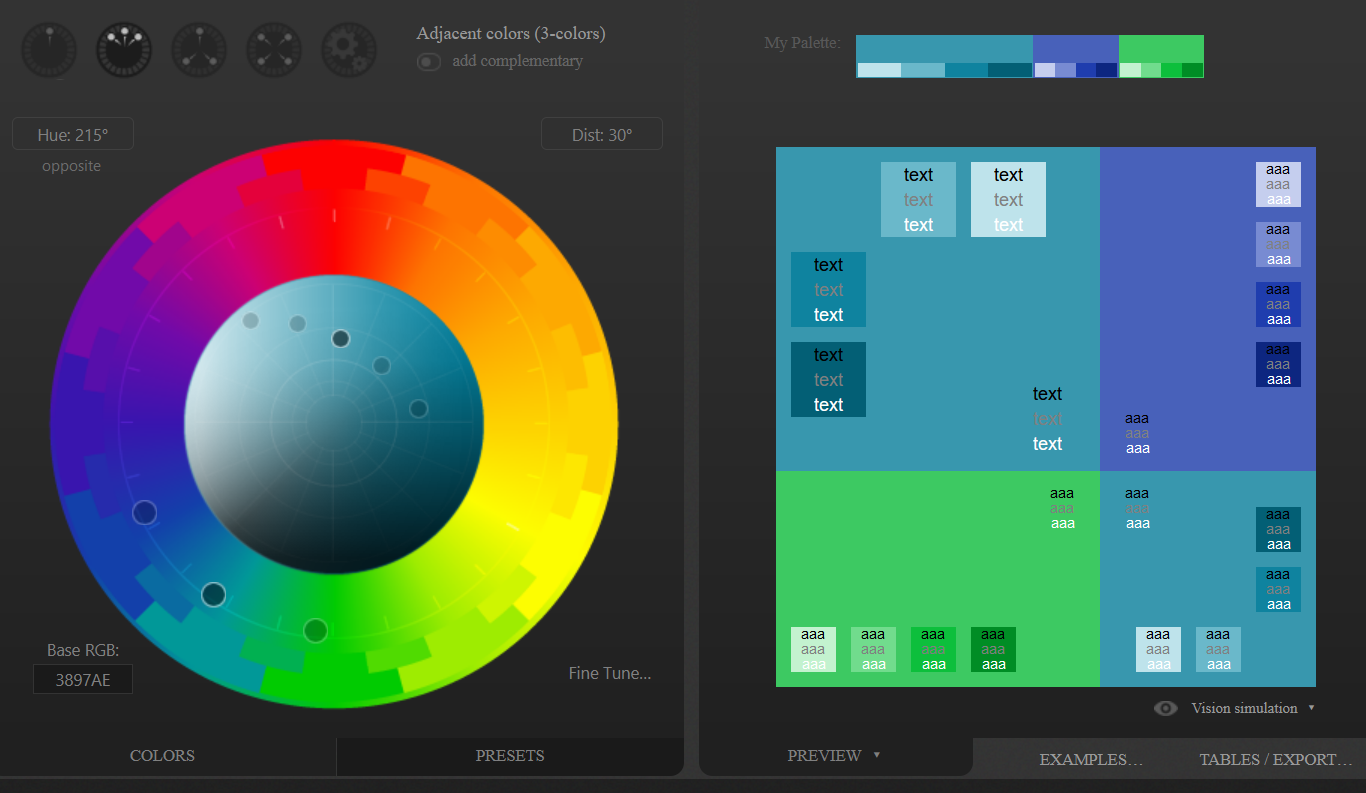
\includegraphics[width=0.8\linewidth]{figures/color-scheme.png}
\caption{Color scheme}
\label{fig:color-scheme}
\end{figure}

\begin{figure}[bh]
    \centering
    \begin{subfigure}[b]{0.4\linewidth}
        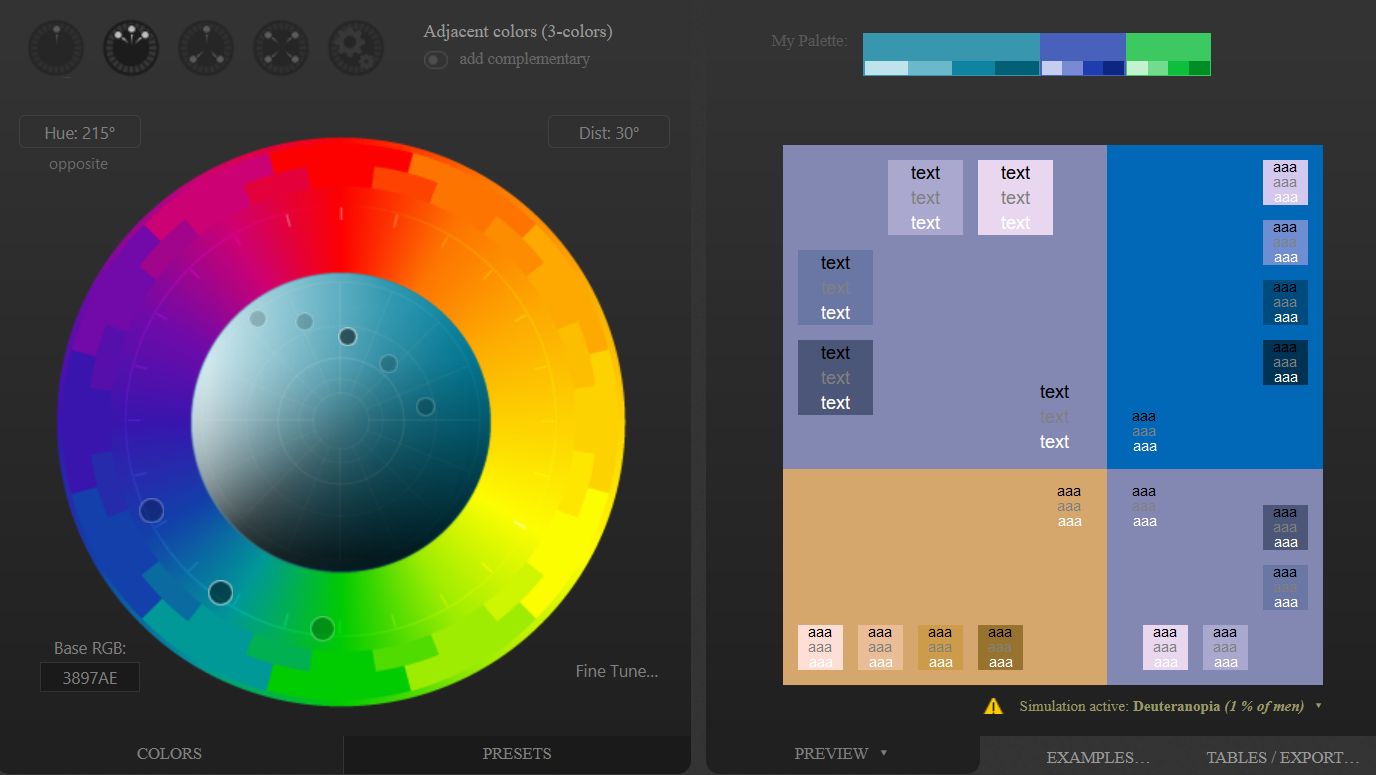
\includegraphics[width=\linewidth]{figures/color-scheme-deuteranopia.png}
        \caption{Deuteranopia}
    \end{subfigure}
    \begin{subfigure}[b]{0.4\linewidth}
        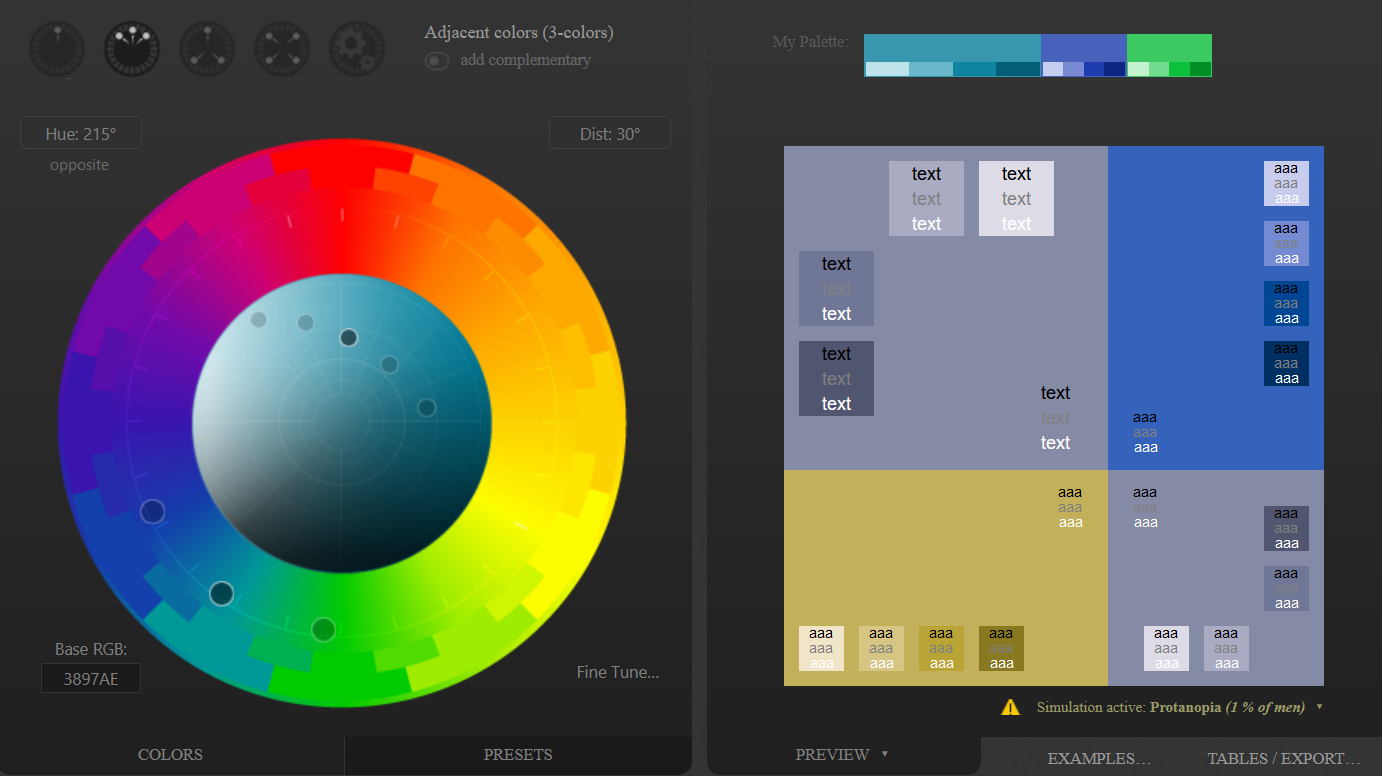
\includegraphics[width=\linewidth]{figures/color-scheme-protanopia.png}
        \caption{Protanopia}
    \end{subfigure}
    \begin{subfigure}[b]{0.4\linewidth}
        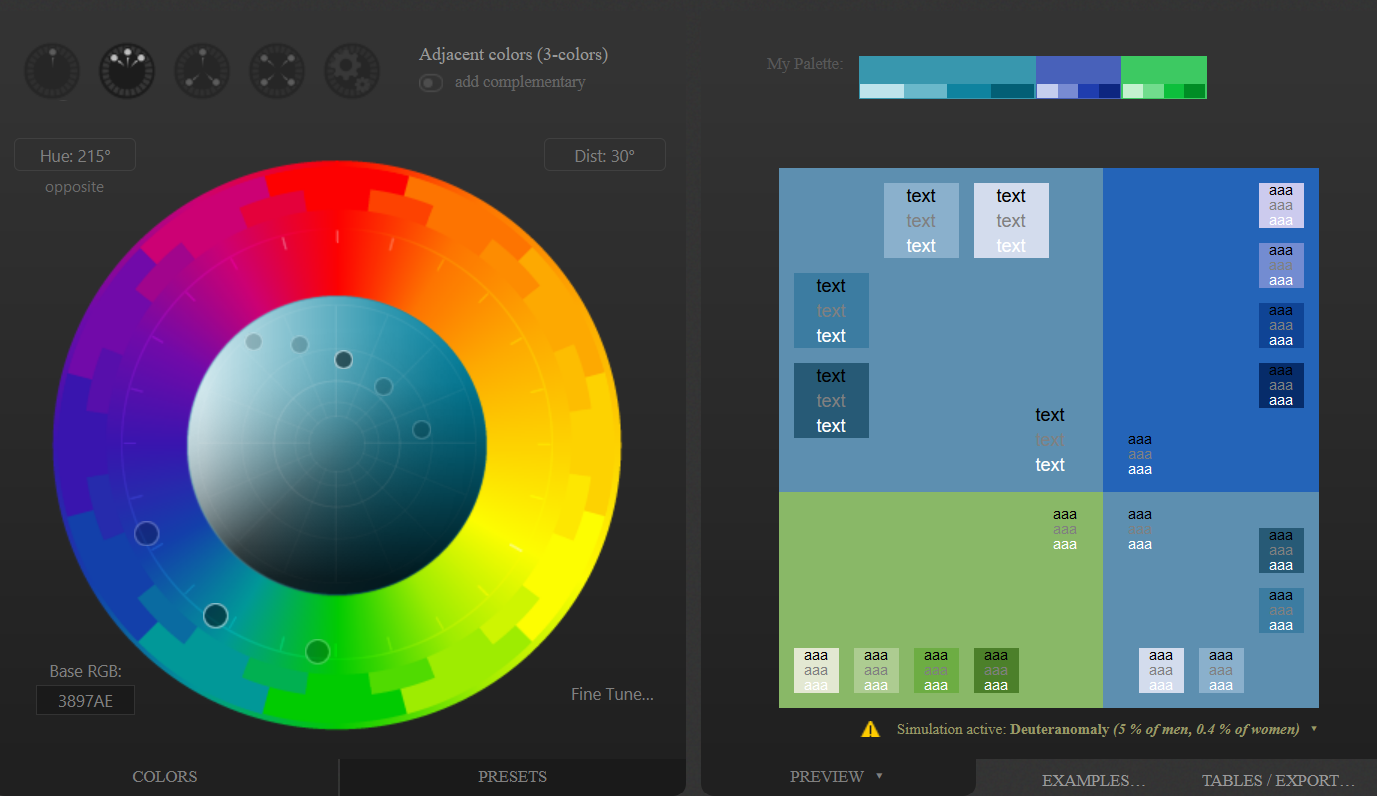
\includegraphics[width=\linewidth]{figures/color-scheme-deuteranomaly.png}
        \caption{Deuteranomaly}
    \end{subfigure}
    \begin{subfigure}[b]{0.4\linewidth}
        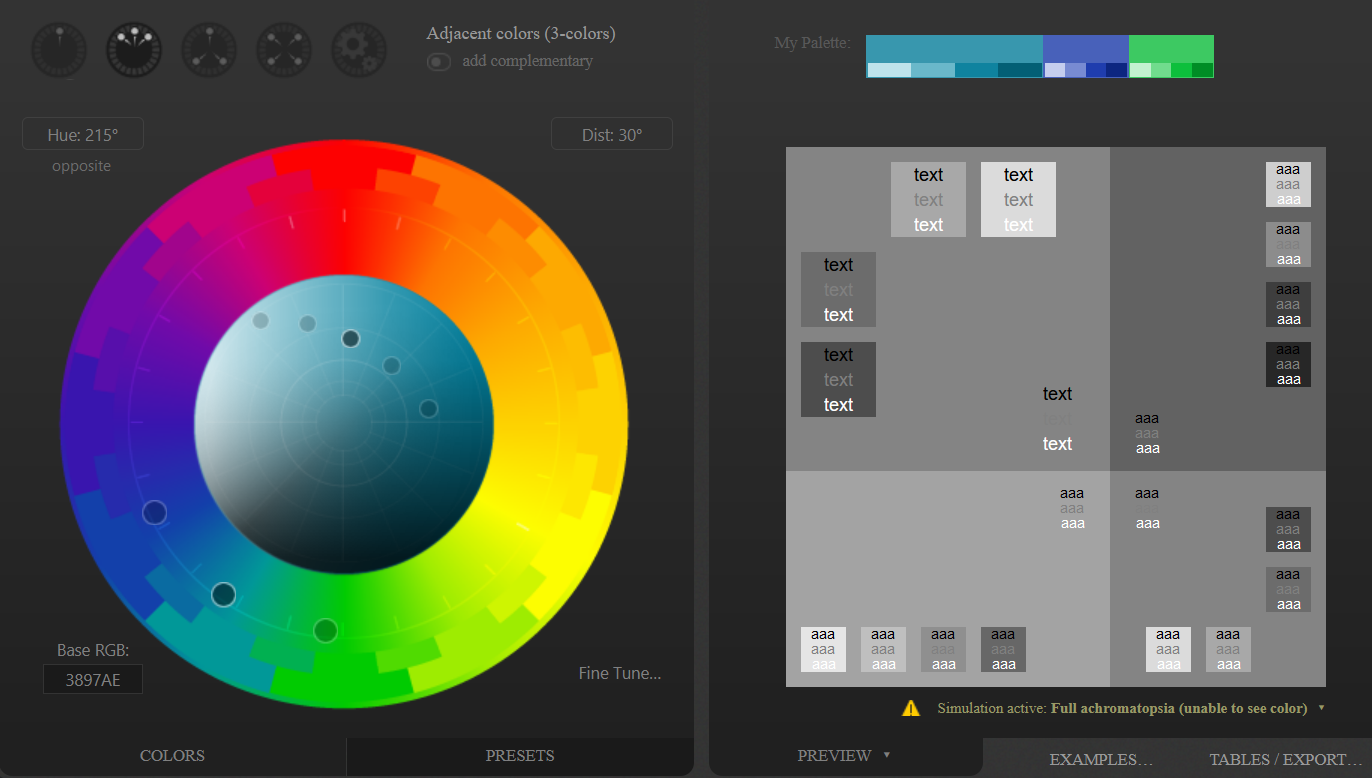
\includegraphics[width=\linewidth]{figures/color-scheme-achromatopsia.png}
        \caption{Achromatopsia}
    \end{subfigure}
\caption{Color Blindness Simulations}
\label{fig:color-scheme-simulations}
\end{figure}